\documentclass[a4paper,12pt]{report}

\usepackage[french]{babel}%langue française
\usepackage[utf8]{inputenc}%encodage des caractères
\usepackage{tikz}
%pour gérer les positionnement d'images
\usepackage{float}
\usepackage{amsmath}
\usepackage{graphicx}
\usepackage[linesnumbered,ruled,french,one language]{algorithm2e}
\makeatletter 
\g@addto@macro{\@algocf@init}{\SetKwInput{KwOut}{Sortie}}
\makeatother
\usepackage{listings}
\usepackage[colorinlistoftodos]{todonotes}
\usepackage{url}
%pour les informations sur un document compilé en PDF et les liens externes / internes
\usepackage[pdftex,hidelinks]{hyperref}
%pour la mise en page des tableaux
\usepackage{array}
\usepackage{tabularx}
%pour utiliser \floatbarrier

%espacement entre les lignes
\usepackage{setspace}
%modifier la mise en page de l'abstract
\usepackage{abstract}
%police et mise en page (marges) du document
\usepackage[T1]{fontenc}
\usepackage[top=2cm, bottom=2cm, left=2cm, right=2cm]{geometry}
%Pour les galerie d'images
\usepackage[most]{tcolorbox}


%-------------------------Informations générale ----------------------------------------
%\makeatletter
%\renewcommand{\@chapapp}{}
%\makeatother

\begin{document}




%régler l'espacement entre les lignes
\newcommand{\HRule}{\rule{\linewidth}{0.5mm}}
\begin{titlepage}
\begin{center}

% Upper part of the page. The '~' is needed because only works if a paragraph has started.

\includegraphics[width=0.35\textwidth]{images/logo}~\\[1cm]

\textsc{\LARGE Licence 2 Informatique}\\[1.5cm]

\textsc{\Large }\\[0.5cm]

% Title
\HRule \\[0.4cm]

{\huge \bfseries Générateur de flores ludiques\\
L-Système \\[0.4cm] }

\HRule \\[1.5cm]

% Author and supervisor
\begin{minipage}{0.4\textwidth}
\begin{flushleft} \large
\emph{\bfseries Auteur:}\\
DIALLO \textsc{Elhadj Alseiny}\\
DJIGUINE \textsc{Mamady}\\
DIALLO \textsc{Abdoulaye Djibril}\\
DIALLO \textsc{Mamadou Alpha}
\end{flushleft}
\end{minipage}
\begin{minipage}{0.4\textwidth}
\begin{flushright} \large
\emph{\bfseries Chargé du cours:} \\
Bonnet \textsc{Grégory}\\
\emph{Encadrant TP:} \\
Dauprat \textsc{Quentin}
\end{flushright}
\end{minipage}

\vfill

% Bottom of the page
{\large \today}

\end{center}
\end{titlepage}
%\thispagestyle{empty}
%\setcounter{page}{0}
\newpage

\tableofcontents
\thispagestyle{empty}
%\setcounter{page}{0}
%ne pas numéroter le sommaire



%espacement entre les lignes d'un tableau
\renewcommand{\arraystretch}{1.5}

%-----------------inclusion des pages----------------------
%thispagestyle{empty}
%recommencer la numérotation des pages à "1"
%\setcounter{page}{0}
%\newpage
\chapter{Introduction}
%\addcontentsline{toc}{chapter}{Introduction}
\section{Sujet et Grandes Lignes}
	Dans toute entité de quelque nature que ce soit ,le travail en équipe s’avère
indispensable entre les personnes qui la composent afin de parvenir à un
meilleur résultat , c’est dans ce cadre qu’il nous a été proposé plusieurs sujets
afin de travailler en un groupe de quatre (4) étudiants sur un de ces sujets et
réaliser une application bout en bout dans un environnement orienté objet
(java) en appliquant les notions de la programmation orientée objet et ses
principes vues durant tout le semestre et plus particulièrement en conception
de logicielle.
\vspace{0.2cm}
Parmi Les sujets proposés celui qui a le plus retenu notre attention est le
Générateur de flores vidéos-ludiques dont l’énoncé est ci-dessous :
\vspace{0.2cm}
« Il n’est pas rare de rencontrer des arbres, buissons ou plantes, plus ou
moins réelles, dans des jeux vidéos ou des films d’animation. Les L-systèmes
permettent de représenter ces modèles végétaux sous formes de système de
réécriture. Le but de ce projet est donc de réaliser un simulateur de L-système
végétal qui prend des règles de réécritures en entrée et produit une image 2D
(ou une scène 3D dans un second temps) de l’objet obtenu par la simulation de ce système. Il faudra donc implémenter un parseur de L-système, un
moteur de réécriture, puis un moteur de rendu graphique pour visualiser ces
plantes. »
Les grandes lignes de ce sujet étant :
\vspace{0.2cm}
\begin{itemize}
	\item Implémentation d’un parseur de l-système permettant de représenter
tout lsystème végétal;
	\item  Faire un rendu 2D en fonction du résultat de réécriture issue de la
génération d’un l-système;
	\item  Et en fin produire la même représentation en scène de 3D .
\end{itemize}

\newpage
\section{Mise en Place du projet}

Pour la mise en place du projet ,nous nous sommes dans un premier orienté dans une optique de compréhension générale des L-systèmes particulièrement un l-système végétal grâce aux liens proposés en dessous du sujet dont le second proposant un livre \textbf{"The algorithmic beauty of plants"}  disponible en ligne décrivant tous les l-systèmes afin de pouvoir adopter un modèle nous permettant de mettre en
place notre parseur et notre modèle de réécriture.
\\
Ensuite nous nous sommes
renseignés sur les différents moteurs de rendu graphique 2D et 3D dont notre
choix s’est finalement porté sur java graphique 2D pour le rendu 2D et JOGL\footnote{(Java Open Graphics Library)}
pour le rendu 3D proposé en dessous du sujet.
\\
\\
 Après avoir compris le vif du sujet ,nous avons décidé de démarrer le projet
selon un ordre de priorité nous permettant d’avancer de façon à mieux gérer notre
temps ,en commençant par le parseur et son modèle de réécriture , le moteur
de rendu 2D et l’interface graphique avec une option aide décrivant notre l-
système pour un usage facile.
\\
\\
En fin nous nous sommes tous focalisé  sur la dernièrement partie qui concerne le rendu 3D .

Notre objectif étant de réaliser un rendu 2D et 3D comme illustrent les deux images suivantes: 
    
    \begin{figure}[h]
        \vspace{5.5em}
        \centering
        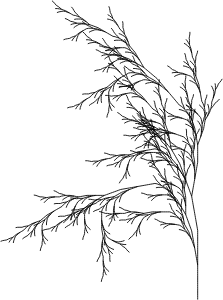
\includegraphics[scale=0.7]{images/tree-one.png}
        \hspace{5.5em}
        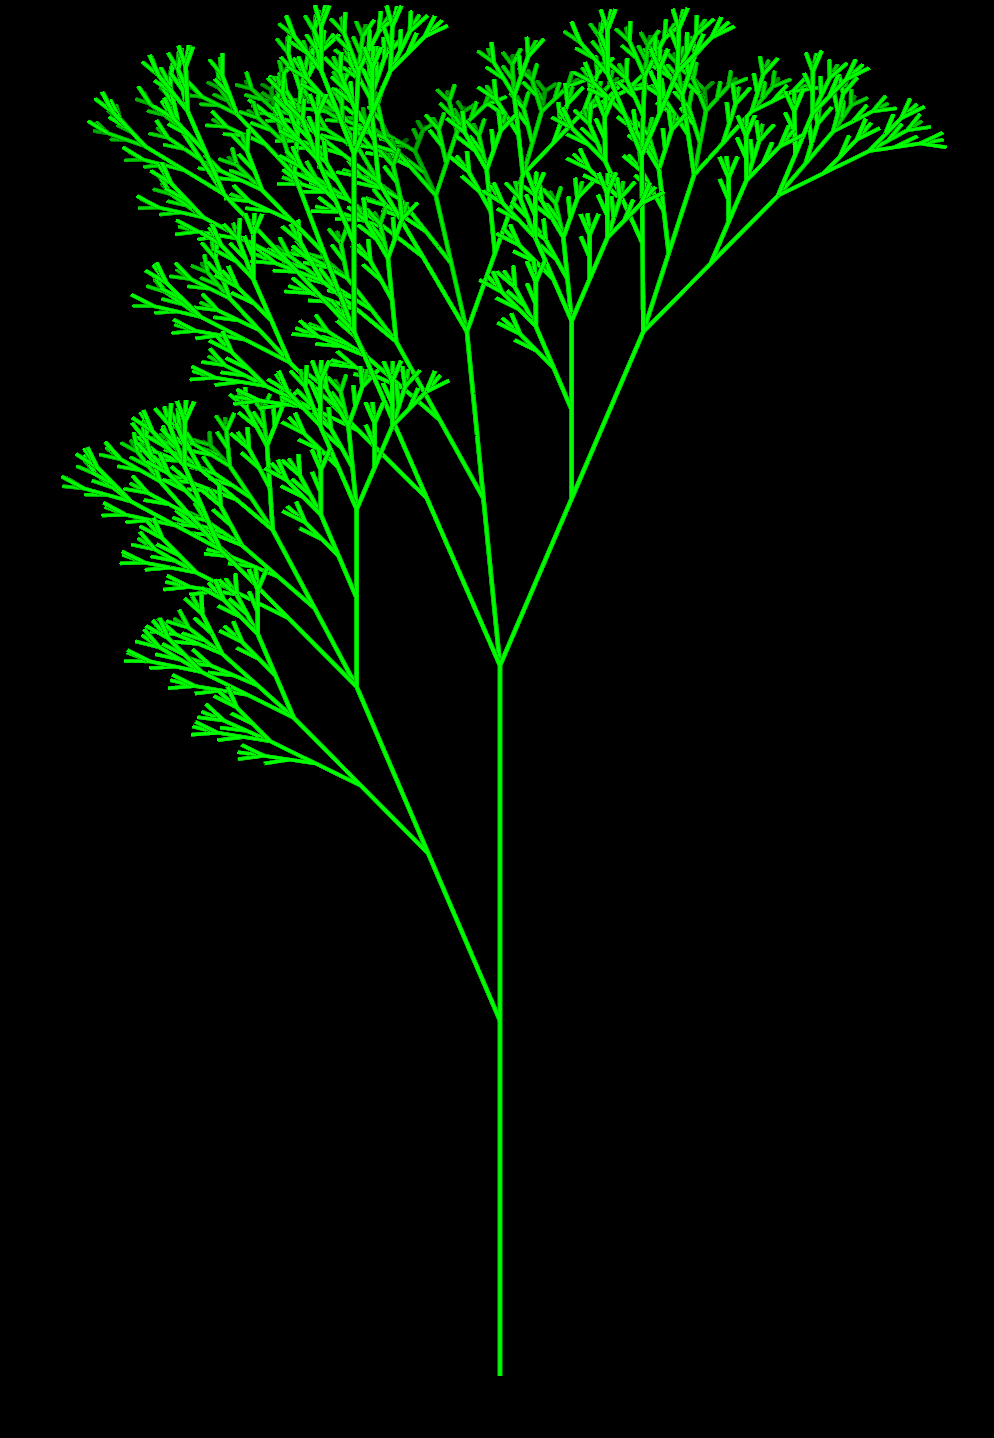
\includegraphics[scale=0.3]{images/tree-two.png}
        \caption{Arbre en 2D et Arbre en 3D}
        \label{fig:my_label}
    \end{figure}
    
	
\chapter{L-Système}
%\addcontentsline{toc}{chapter}{L-Système}
\section{Définition et Fonctionnement}

\subsection{De quoi s’agit-il ?}	
Un L-System (ou système de Lindenmayer) inventé en 1968 par le biologiste
hongrois Aristid Lindenmayer \footnote{Lindenmayer Biologiste hongrois} est un ensemble de règles et de symboles
qui modélisent un processus de croissance d’êtres vivants comme des plantes ou des cellules.

\subsection{Principe de Fonctionnement}
	Un L-système est un système de réécriture qui comprend : 
	\vspace{0.2cm}
\begin{itemize}
	\item \textbf {Un alphabet :} l’ensemble des variables et constantes du L-Système;
	\item \textbf{Un axiome :} qui représente le point de départ c’est à dire l’état initial.
	\item \textbf {Un ensemble de règles :} permettant à chaque étape de substituer les variables par leurs correspondants.
	\vspace{0.2cm}
	Ainsi ,on obtient un L-système part toujours d’un axiome de départ avec
un ensemble de règle qui vont être appliquée à chaque itération (entier de
valeur donnée) jusqu’à trouver le mot résultat par substitution et qui sera
ensuite interprété pour être interprété sous forme de rendu graphique 2D ou
3D
\end{itemize}		
	 
 
\section{L-Système Utilisé}
Un l-système étant essentiellement composé de lettres et symboles, notre l-
système végétal utilise les lettres de l’alphabet et des symboles ci-dessous :

\begin{table}[h]
      \centering
      \begin{tabular}{|c|c|}
           \hline \textbf{Symboles} & \textbf{Interprétations} \\ \hline
           \{LETTRE\}\textbackslash \{H,B\} & Avancer d’une unité (dessine une branche) \\ \hline
            + & Tourner à gauche d’un angle \\ \hline
            - & Tourner à droite d’un angle \\ \hline
            [ & Enregistrer la position et l’orientation \\ \hline
            ] & Rétablir la positon et l’orientation  \\  \hline
            > & Rouler à gauche d'un angle $\alpha$  \\  \hline
            < & Rouler à droite d'un angle  $\alpha$ \\  \hline
            B & S'incliner vers le bas en 3D \\  \hline
            H & S'incliner vers le haut en 3D \\  \hline
            \hline
      \end{tabular}
      \caption{Interprétations des symboles}
      \label{tab:my_label}
  \end{table}
\newpage
Nous avons proposé beaucoup d’exemples de L-system végétal
afin d’illustrer plusieurs exemples dont entre autres nous avons :
  
  \begin{table}[h]
   Pour un nombre de trois d'itération appliqué a au système ci-haut le tableau ci-dessous détaille 
le résultat obtenue  à chaque itération par application de la règle .
\\
\\
  		\centering 
  	
	\begin{tikzpicture}
	\node  (base gauche) at (-3,0) {Axiome de Base:};
	\node (base droite) at  (2,0) {X};
	\node (regle1 gauche) at (-3,-1) {Règle1:};
	\node (regle1 droite) at (1,-1) {X={F[+X][-X]FX}};
	\node (regle2 gauche) at (-3,-2) {Règle2:};
	\node (regle2 droite) at (1,-2) {F=FF};
	\node (it0 gauche) at (-5,-3) {iteration 0};
	\node (it0 droite) at (2,-3) {F[+X][-X]FX};
	\node (it1 gauche) at (-5,-4){iteration1};
	\node (it1 droite) at (2,-4){FF[+F[+X][-X]FX][-F[+X][-X]FX]FFF[+X][-X]FX};
	\node (it2 gauche) at (-5,-5) {iteration2};
	\node (it2 droite) at (2,-5) { FFFF[+FF[+F[+X][-X]FX][-F[+X][-X]FX]FFF[+X][-X]};
	\node (it2 droite suite1) at (2,-6) {FX][-FF[+F[+X][-X]FX][-F[+X][-X]FX]FFF[+X][-X]FX]};
	\node (it2 droite suite2) at (2,-7){FFFFFF[+F[+X][-X]FX][-F[+X][-X]FX]FFF[+X][-X]FX};
	\end{tikzpicture}
	\caption{Exemple de génération}\label{figure}

  \end{table}

\chapter{Organisation du Projet}
\section{Répartition des taches}

Le projet étant essentiellement composé de trois grandes parties ,nous
nous sommes dans un premier temps réunis afin de mieux comprendre le
sujet et élaborer un plan de travail ,ce qui nous a permis de comprendre c'est quoi un l-système dans l’ensemble, de quoi a t on besoin pour le représenter mais
aussi la notion de réécriture qui est fonction d'un axiome, d’un ensemble règles  et un
nombre d’itération puis en denier nous avons aussi appris des notions d'interprétation
de représentation du résultat de ce système de réécriture sous de rendu graphique 2D et 3D.
\\
Mamady Djiguiné s’est chargé de développer le parseur et l’écriture de son
test, pendant ce temps Abdoulaye Djibril travaillait sur la représentation
en 2D grâce aux exemples de génération donné dans le livre \textbf{"The algorithmic beauty of plants"},de même Diallo Alseiny travaillait quand à lui sur l’interface graphique et le rendu 3D; en fin Mamadou alpha Diallo s’est chargé de préparer les fichiers indispensables pour une bonne configuration de notre application
(Ant ,manifeste) mais aussi du rapport de notre projet.

\section{Architecture du Programme}
Concernant l’architecture de notre projet, nous avons voulu la relier au
sujet pour une compréhension facile.Cependant nous avons opté pour une
décomposition en quatre (4) packages:
\\
\begin{itemize}
	\item \textbf{parser : }le package parser permet de générer un l-système sous forme de chaîné de caractères ;
	\\
	\item \textbf{graphique :}permet d’interpréter le résultat du parser en rendu 2D et 3D;
	\\
	\item \textbf{utils : } permet de gérer les différents positionnement au niveau du rendu ;
	\\
	\item \textbf{interfaceuser :}  gérant tout ce qui est interface graphique utilisateur.
\end{itemize}

\newpage
\begin{figure}[t]
		\centering
		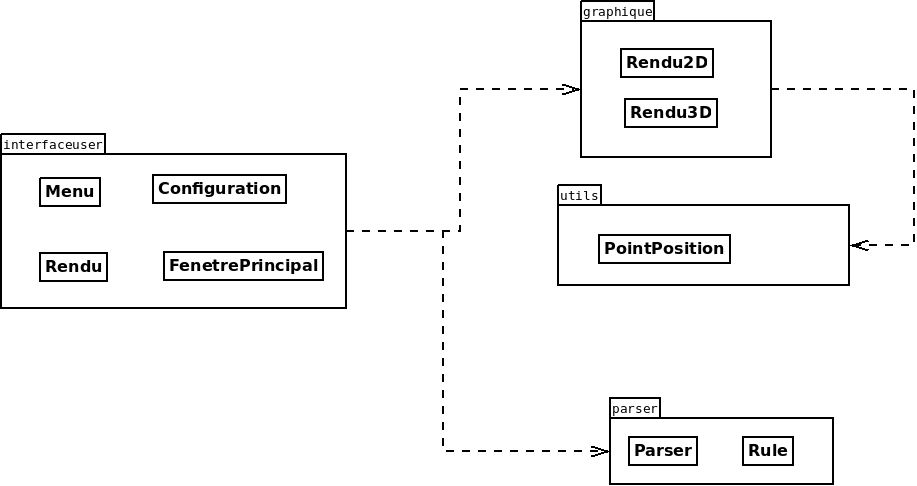
\includegraphics[width=16cm]{images/package.png}
	    \caption{Diagramme des packages }
\end{figure}
\begin{figure}[h]
		\centering
		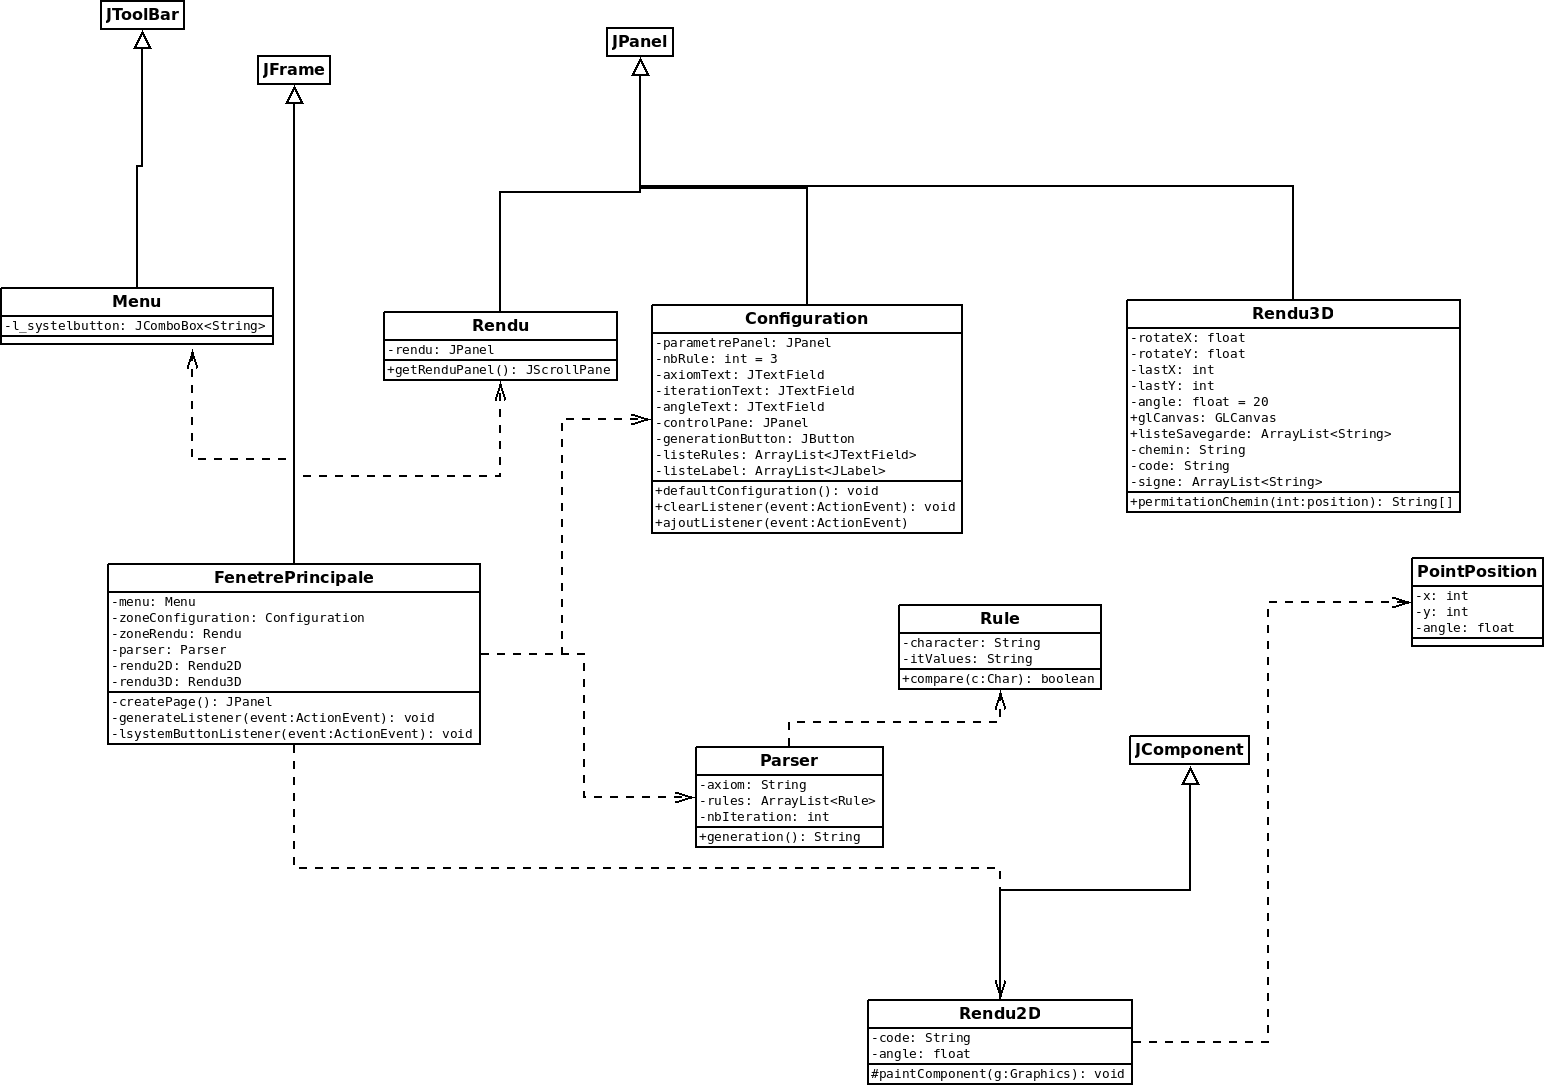
\includegraphics[width=18cm]{images/classe.png}
	    \caption{Diagramme des Classes }
\end{figure}

\chapter{Élément Technique}
%\addcontentsline{toc}{chapter}{Élément Technique}
\section{Parseur}
le parseur comme son nom l'indique constitue le cœur de notre application grâce à sa méthode 
génération permet de produire une chaîne  représentant un l-système végétal par réécriture en se servant d'un axiom de départ,un nombre d'itération  et des règles créée à partir de la classe \textbf{\em Rule} qu'il contient sous forme de liste .
\\
Pour qu'elle produise une chaîne représentant un l-système il faut se s'assurer que ses attributs aient été initialisés et qu'aucun d'entre eux  ne soit nul pour ceux de type entier et non vide pour ceux de type chaîne.En plus de ses attributs sa méthodes génération se sert également d'une méthode \textbf{\em compare} pour substituée chaque caractère par la chaîne devant le substituer suivant les règles définies.
\\
\\
l'algorithme de la génération d'un l-système par réécriture 
\\
	\begin{algorithm}
		\DontPrintSemicolon 
		\caption {Génération d'un l-système par réécriture  }
		\KwIn {axiom: $String$ , rules: $List[Rule]$ , nbIteration: $Integer$}
		\KwOut {Chaîne complète après la dernière itération}
		\For {$i \gets 0$ \textbf{à} $nbIteration$}{
				$production \leftarrow "" $ \;
				\For {$j \gets 0$ \textbf{à} $axiom.taille$}{
					$hasBeenUpdated \leftarrow faux $ \;
					\For {$Rule \ $r : $rules$}{
						\If{ $r.compare (axiom.charAt[j])$}{
							$hasBeenUpdated \leftarrow vrai $\;
							$production \leftarrow production + r.getItValues{} $ \;
							$arreter $\;
						}
					}
					\If{$!hasBeenUpdated $}{
							$production \leftarrow $production + $axiom.charAt[j] $ \;
					}
				}
				$axiom \leftarrow production $\;
		}
		\Return {$axiom$}\;
	\end{algorithm}
\section{Rule}
Elle permet de composer les règles d'un l-système  que la classe parser utilisera pour produire un system sous forme de chaîne avant que cette dernière ne soit interprétée  sous forme de rendu 2D ou 3D.Cette classe est très utile aussi car elle contient en son sein une méthode \textbf{\em compare} qui prends un caractère et retourne la chaîne devant le substituer lors d'une génération.


\section{Interface}
Nous avons utilisé l'interface java swing pour realiser l'interface utilisateur de notre application .Elle composée quatre (4) classes.
une permettant d'afficher la fenetre principale,une autre permettant de faire les Menu ,une troisième permettant defaire tout ce qui est configuration .

\subsection{FenetrePrincipale:}	
	Rassemble  tous les composants graphiques  menu,configuration et rendu. Elle constitue l'élément centrale gérant le lien entre le parseur et les modes de rendu.
\subsection{Configuration:}	\label{config}
	Définie les zones de paramétrage de l'application ainsi que les boutons de contrôle:
	\begin{itemize}
		 \item \textbf{Générate:} permettant générer un rendu 2D ou 3D du l-système;
		 \item \textbf{newRule:} pour ajouter au tant de règles souhaitées;
		 \item \textbf{clear:}  pour nettoyer les zone de textes et rendu .
	\end{itemize}
\subsection{Menu:}	
	Contient une liste déroulante de quelques exemples de l-systèmes sous format 2D et 3D, ainsi que l'option aide qui explique le fonctionnement du système. 
\subsection{Rendu:}
 Contient deux cases à cocher \textbf{rendu2d}, \textbf{rendu3d} permettant de choisir un mode de rendu ainsi qu'une zone de rendu pour la visualisation.
\section{Moteur graphique}
En ce qui concerne nos moteurs de rendu, nous utilisons du java swing pour le rendu 2D et jogl (java open gl library ) pour le rendu 3D .
	
\subsection{Rendu2D}
Nous utilisons du java swing pour faire le rendu 2D en redéfinissant la méthode \textbf{\textit{paintComponent(graphics 2d)}} de celui-ci. g2d.drawLine pour tracer les lignes(branche), g2d.translate pour faire des translations, g2d.scale pour gérer la mise en gras et une liste pour sauvegarder les positions si nécessaire.
\newpage
	\begin{figure}[h]
		 \centering
		 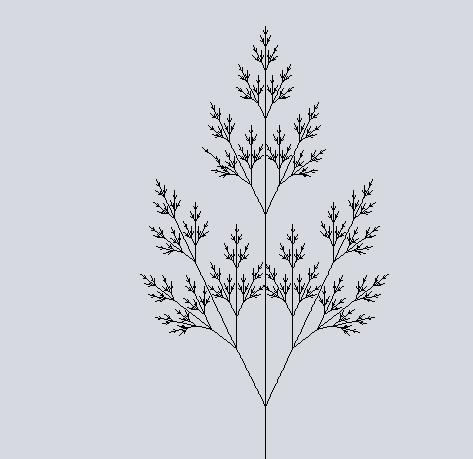
\includegraphics[width=7cm]{images/arbre2D.jpeg}
		 \caption{Exemple de rendu 2D}
		\end{figure}
	
\subsection{Rendu3D}
Comme mentionner ci-dessus, nous utilisons java openGL library pour faire notre rendu 3D notamment: gl2 pour afficher les lignes
glu pour placer la caméra et GLUT pour afficher les cylindres.
GLCanvas crée la fenêtre, GLEventListener initialise et affiche l’environnement 3D.
\\
	\begin{figure}[h]
		\centering
		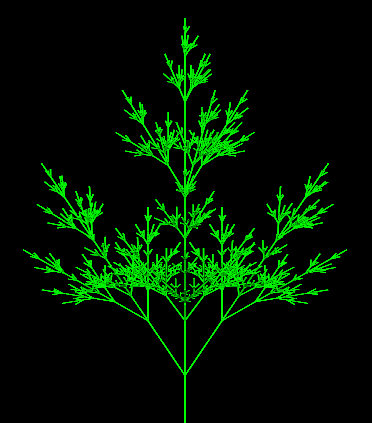
\includegraphics[width=7cm]{images/arbre3D.png}
	    \caption{Exemple de rendu 3D }
    \end{figure}
    	

\chapter{Expérimentations et Usages}
\section{Utilisation}
	Notre avons développé notre application avec du java standard Édition 11 pour des raisons compatibilité avec les ordinateurs de l'université. Elle peut s'exécuter sur les distributions Linux avec interface graphique tel que Ubuntu version 20.04.4 LTS, sur mac Os 12.3.1 et windows 10.
	
\section{Lancement de l'application}
 	Vous devez ouvrir un terminal à l'emplacement du dossier .
 	\\ \\
 	Pour :
 	\begin{itemize}
 		\item Lancer l'application exécuter : \fbox{ \textbf{\em ant run}} ou \fbox{ \textbf{\em ./scripts/run.sh}}
 		\item Initialiser le projet: \fbox{\textbf{\em ant init}}  ou fbox{\textbf{\em ./scripts/install.sh}} \\
 			Cette initialisation créera  les dossiers de bases  bin, doc et dist 
 		\item Compiler le projet: \fbox{\textbf{\em ant compile}} ou \fbox{\textbf{\em ./scripts/compile.sh}}
 		\item Générer le Javadoc: \fbox{\textbf{\em ant javadoc}} ou \fbox{\textbf{./scripts/makedoc.sh}}		
 		\item Générer le fichier jar: \fbox{\textbf{\em ant packaging}} ou \fbox{\textbf{\em ./scripts/makejar.sh}}
 		\item Exécuter le fichier jar:\fbox{\textbf{\em ./scripts/	runjar.sh}}
 		\item Nettoyer le projet: \fbox{\textbf{\em ant clean}} ou \fbox{\textbf{\em ./scripts/clean.sh}}
 		\item Lancer le test: \fbox{\textbf{\em ant test}} ou \fbox{\textbf{\em ./scripts/test.sh}}
	\end{itemize} 		
 	
\section{Fonctionnement de l'interface Graphique}
	Au lancement du programme, il se présente avec un exemple par défaut visualisable  
par clic sur le bouton \textbf{Generate} sous forme 2D ou 3D.\\
	Dans la barre de menu existe une liste déroulante contenant d'autres exemples ainsi qu'un bouton aide permettant à l'utilisateur de mieux comprendre le fonctionnement de l'interface et l'interprétation des symboles.

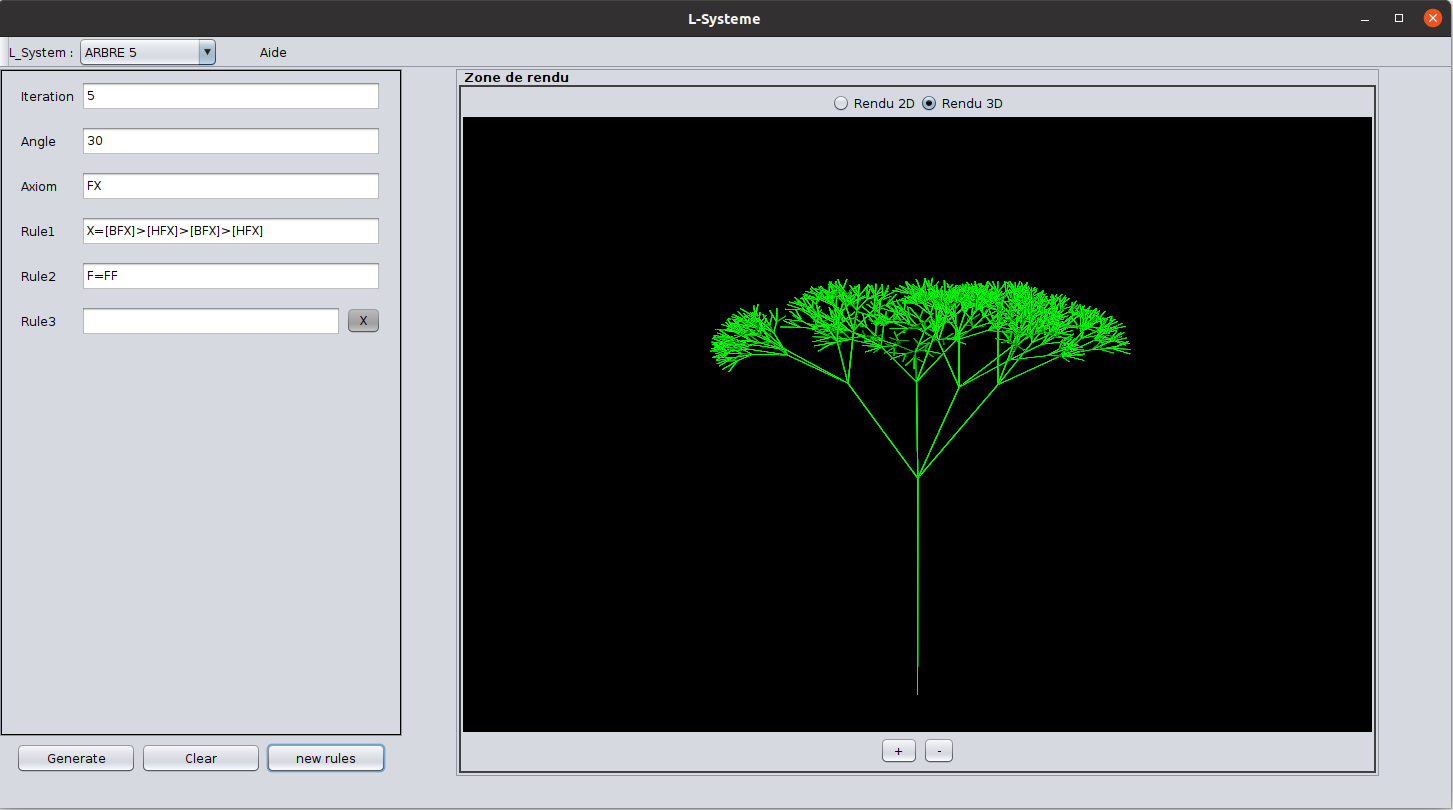
\includegraphics[width=16cm]{images/interface.png}
\\
\\
Il est possible qu'un utilisateur puisse composer ses  propres règles. Pour cela les boutons \textbf{ clear, Generate} et \textbf{Newrule} lui sera d'une aide (voir Configuration~\ref{config} page \pageref{config}) pour l'utilisation des ces boutons.

Attention  l'application tient compte de la caste. Toute modification entraînée sur l'interface graphique il faudrait cliquez sur le bouton \textbf{Generate} pour la visualiser.

Dans la zone rendu  à gauche le rendu 2d est coché par défaut est vous pouvez le remettre sur le rendu 3D. 

%En 3D des éléments supplémentaires sont ajoutées aux règles .
\section{Navigation dans l'interface graphique 3D}

Pour naviguer dans l'espace 3D les boutons : + ou - serviraient à zoomer  ou dézoomer respectivement.
\\
\begin{itemize}
	\item Bouton \textbf{+} permet de zoomer
	\item Bouton \textbf{-}  permet de dézoomer 
\end{itemize}

En plus un clic glissé de la souris :
\begin{itemize}
	\item Vers la droite : permet de faire tourner l'arbre autour de lui même dans la même direction;
	\item Vers la gauche: permet de faire tourner l'arbre  autour de lui même dans la même direction ;
	\item Vers le bas: incline l'arbre vers le bas 
\end{itemize}
\newpage
\section{Test du logiciel}
\subsection{Possible problème}
	Lorsque vous lancer et essayer de générer un arbre avec un nombre d'itération au delà d'un certain seuil suivant la composition de l'arbre, cela pourrait prendre un peu de temps pour le parseur lors de la réécriture et sa représentation 3D voir 2D pourrait déborder. Dans ce cas une solution serait de diminuer le nombre d'itération, en plus en 3D on pourrait aussi dézoomer.

\subsection{Test du logiciel}
	Nous avons réalisé nos tests en utilisant le framework open source \textbf{Junit-4.12} le développement et l'exécution de tests unitaires. Elle teste l'ensemble des méthodes indispensables pour la réécriture d'un arbre.
\\ 
	\begin{figure}[h]
		\centering
		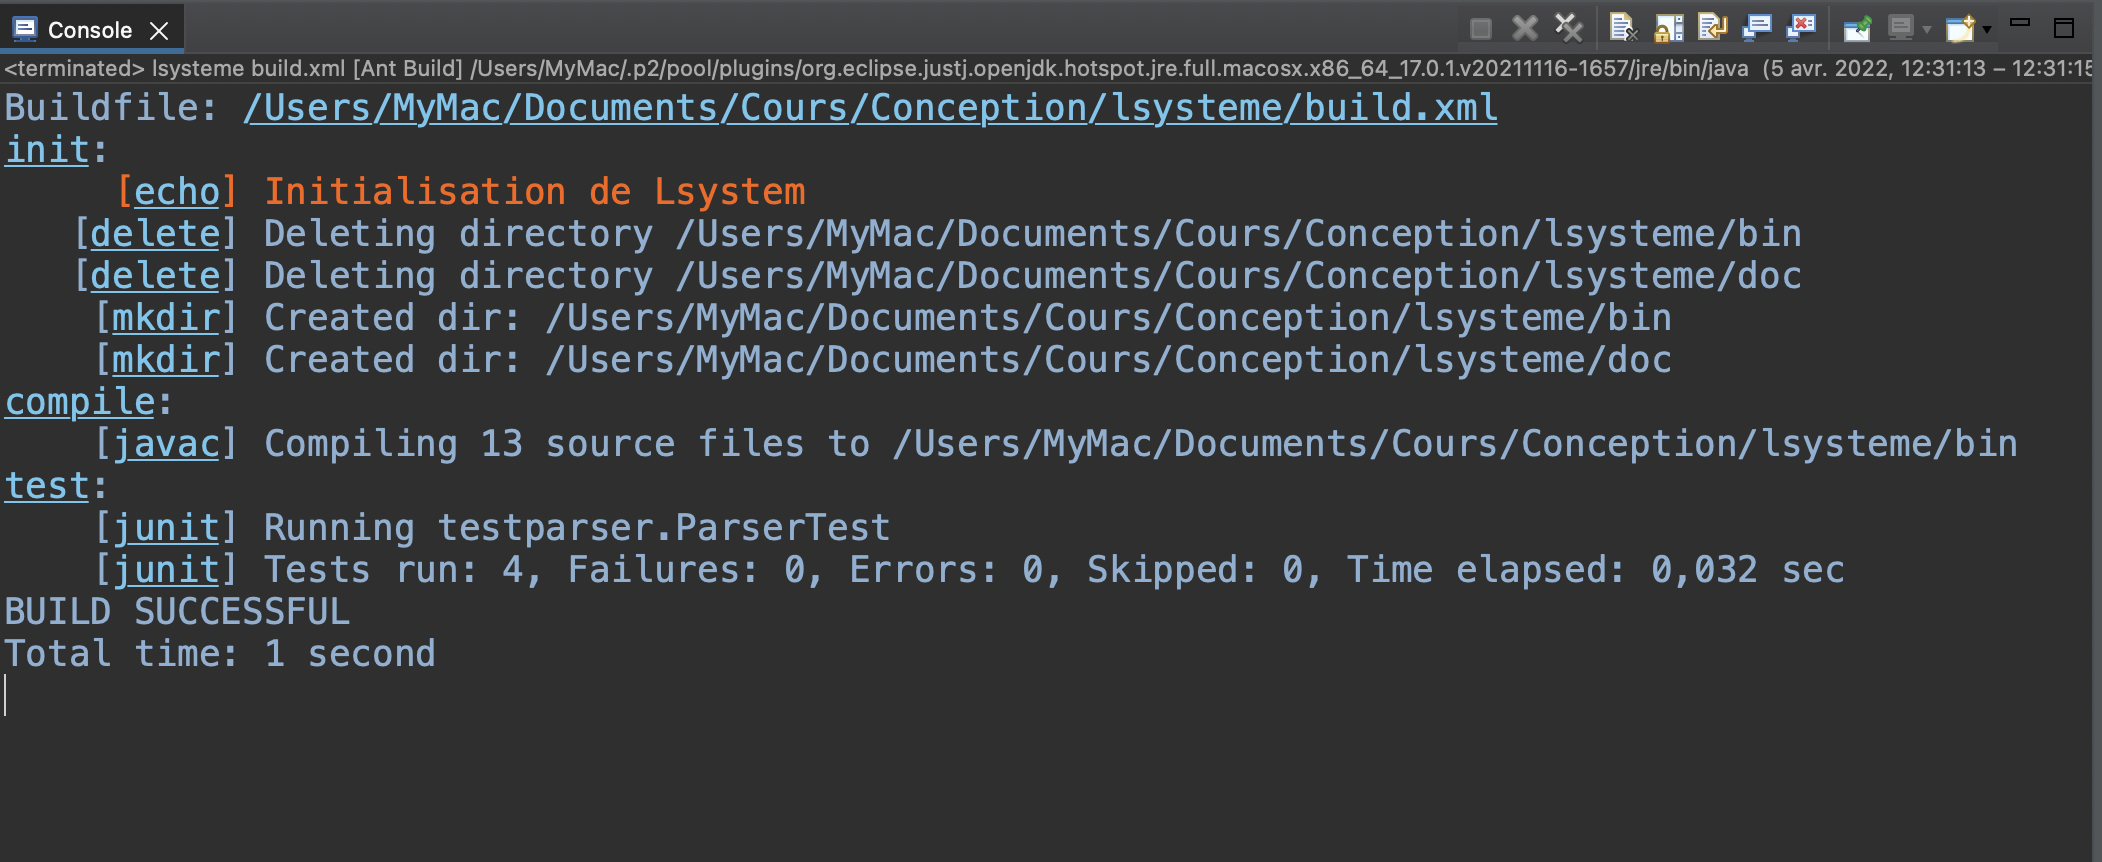
\includegraphics[width=16cm]{images/test.png}
	    \caption{Test }
	\end{figure}
\chapter{Conclusion}

\section{Bilan de nos travaux}
	Étudier un sujet aussi passionnant que le l-système. Nous avons appris beaucoup de chose dans ce vaste domaine allant d'une expérience de modélisation aux différentes étape de création d'un arbre en passant par des exercices de programmation en Java. 
	Il était très agréable de voir les idée théorique se concrétiser en rendu 2D et 3D. Nous retenons également de ce projet, la nécessité d’une bonne préparation, l’importance de la recherche et la gestion du temps pour la réalisation d’un programme.
	
\section{Améliorations possibles}

Nous pouvons continuer ce projet en de nombreuses façon :  
\begin{itemize}
	\item On aurait pu implémenter des l-système paramétrique et faire réagir l'arbre avec son environnement 
	\item colorisation des arbre en 2D et 3D
	\item Possibilité d'ajouter plusieurs arbres dans la même fenêtre cote à cote
	\item Généraliser l'étude afin de pouvoir représenter n'importe quel l-système
	\item Implémenter des stochastiques l-système
	\item Ajouter des contrôles clavier sur le rendu 3D 
\end{itemize}

\begin{thebibliography}{1}
		\bibitem{notes} Wikipedia L-Système (FR): {\em https://fr.wikipedia.org/wiki/L-Système} .
		\bibitem{notes} Wikipedia L-Système (EN): {\em https://en.wikipedia.org/wiki/L-system} .
		\bibitem{norman} E. H. Norman {\em https://www.techno-science.net/definition/11374.html} 		
		\bibitem{fo} Bob Tadashi Wakabayashi {\em https://www.cs.unm.edu/~joel/PaperFoldingFractal/
		L-system-rules.html}
		\bibitem {notes} The algorithmic beauty of plants {\em http://algorithmicbotany.org/papers/abop/abop.pdf}
		\bibitem {note} Moteur de rendu 3D {\em https://jogamp.org/jogl/www/}
		\bibitem {note} JOGL Tutorial { \em https://www.javatpoint.com/jogl-tutorial}
		\bibitem {note} Dessin java et java 2D {\em http://www-igm.univ-mlv.fr/~berstel/Cours/CoursJava/8-Dessin.pdf}
		\bibitem {note} Java Platform Standard Edition 8 Documentation {\em https://docs.oracle.com/javase/8/docs/}
		\bibitem {note} Stack overflow {\em https://stackoverflow.com/questions/18875244/java-build-ant-file-with-external-jar-files}
		\bibitem {note} Houdini {\em https://www.sidefx.com/docs/houdini/nodes/sop/lsystem.html}
		\bibitem {note} L-System Rules Parser {\em http://jeromeetienne.github.io/lsystem-js/parser-tool.html}
		\bibitem {note} Vexlio {https://www.vexlio.com/blog/drawing-simple-organics-with-l-systems/}
		
\end{thebibliography}

\end{document}